\newcommand{\Harmonization}{
  \begin{figure}
    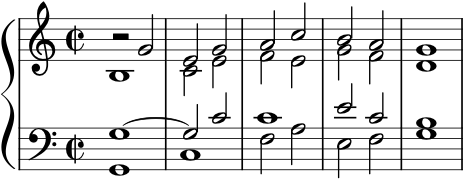
\includegraphics[width=5.5cm]{fig/piston.png}
    \hspace{1cm}
    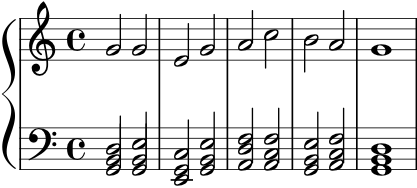
\includegraphics[width=5cm]{fig/fharm.png} \\
    \begin{flushleft}
    \begin{small}
     \hspace{2.35cm} V \ \ \ \ \ \ \ \,I \ \ \ \ \ \ \ \,IV \,VI \ \,III \ IV \ \ \,V
     \hspace{2.6cm} V \ \ \ \ \ \ \ \,I \ \ \ \ \ \,IV VI \,III\,IV \ \ V
    \end{small}
    \end{flushleft}
    \caption{Harmonization by Piston (left) and \fharm (right)}
    \Description{Harmonization by Piston (left) and \fharm (right)}
    \label{fig:harmonization}
  \end{figure}
}

\section{Harmony}
\label{sec:harmony}

Harmony is a particularly fundamental area of music theory with numerous texts, for
example \citet{piston-harmony} and \citet{aldwell2018harmony}, devoted
to it. It has also been the focus of most of the Haskell-based
work~\citep{magalhaes-harmtrace,koops-fharm,magalhaes-fcomp}, and as a
first step into this huge area it worth trying to implement some of
this functionality in Agda. Indeed \citet{magalhaes-harmtrace} states in its final section
``It would be interesting to see if we could easily port our system to
a dependently-typed setting'' and explicitly mentions Agda and Idris
as candidates. Our work, while currently very preliminary, provides a
glipse into what that can look like.

\citet{magalhaes-harmtrace} is devoted to creating a grammar for
harmonic analysis and a corresponding parser that takes as input a
series of chords and tries to produce a harmonic analysis that fits
the progression. The grammar makes crucial use of dependent types and
is thus awkard to represent in Haskell. We have implemented those
parts in Agda and not surprisingly they are simple and
elegant. However \citet{magalhaes-harmtrace} also makes use of
sophisticated Haskell libraries for parser combinators and generics,
which are unavailable in Agda and would either have to be natively
implemented or called through Agda's Haskell FFI, both of which involve
considerable work, so we have not yet pursued that route.

Instead we first focus on FHARM~\citep{koops-fharm}, which aims to create a
harmonize a given melody. This is the subject of Chapter~9 of
\citet{piston-harmony}, and, along with three exercises,
FHARM harmonizes the main Example~9.1 of the chapter,
shown in Figure~\ref{fig:harmonization}.

\Harmonization

Their techinique is to first require the melody notes be members of
the harmonizing chords, then use their previous work to try to
create a harmonic analysis of every possible sequence of chords that
arises, chosing the one that has most closely fits their
grammar. Although the result is not bad, it clearly leaves room for
improvement. Noted in the paper is that no attenton is given to
voicing (how each of the four parts flows horizontally and how the
lines interact---in other words the counterpoint). Not noted is that
the melody note is always doubled, whereas typically in four-part
harmony it is prefered to double the root note. Also mimimizing the
number of parse errors as a means to choose the best harmonization
does not necessarily have a musical meaning.

Not having an impelmentation of the grammar and parser we explore a
different approach, based closer on Piston's own.

TODO: More here.
